\documentclass[a4paper,10pt,draft]{article}%


\usepackage[hidelinks]{hyperref}
\hypersetup{
  % colorlinks,
  final,
  linktoc=page 
}
\usepackage{bookmark}

\input{commands.tex}%

\usepackage[draft]{showkeys}
\usepackage[obeyDraft]{todonotes}
\usepackage{mathtools}  
\mathtoolsset{showonlyrefs}  

\usepackage{fullpage}


%-------- TIKZ -----------------------------------------
\usepackage{tikz}%
\usetikzlibrary{matrix,arrows,decorations.pathmorphing,cd,patterns}
\tikzset{%
  treenode/.style = {shape=rectangle, rounded corners,%
                     draw, align=center,%
                     top color=white, bottom color=blue!20},%
  root/.style     = {treenode, font=\Large, bottom color=red!30},%
  env/.style      = {treenode, font=\ttfamily\normalsize},%
  dummy/.style    = {circle,draw,inner sep=0pt,minimum size=2mm}%
}%

\usetikzlibrary[decorations.pathreplacing]
% \usetikzlibrary{external}\tikzexternalize
% \makeatletters
% \renewcommand{\todo}[2][]{\tikzexternaldisable\@todo[#1]{#2}\tikzexternalenable}
% \makeatother


% --------Background Coloring IFDRAFT--------------------------
\usepackage{ifdraft}
\ifdraft{
  \color[RGB]{63,63,63}
  % \pagecolor[rgb]{0.5,0.5,0.5}
  \pagecolor[RGB]{220,220,204}
  % \color[rgb]{1,1,1}
}


% -------- Referenece Numbering
\numberwithin{equation}{section}%


% ------- Author Info -----------------------

\author{Peter Bonventre, Lu\'is A. Pereira}%
\title{Equivariant dendroidal sets and simplicial operads}%
\date{\today}



%----- Document ---------------------------------



\begin{document}	\maketitle%



\abstract{bla bla, generalizing.

In an appendix, we discuss Reedy categories in the equivariant context.}




     \begin{equation}
            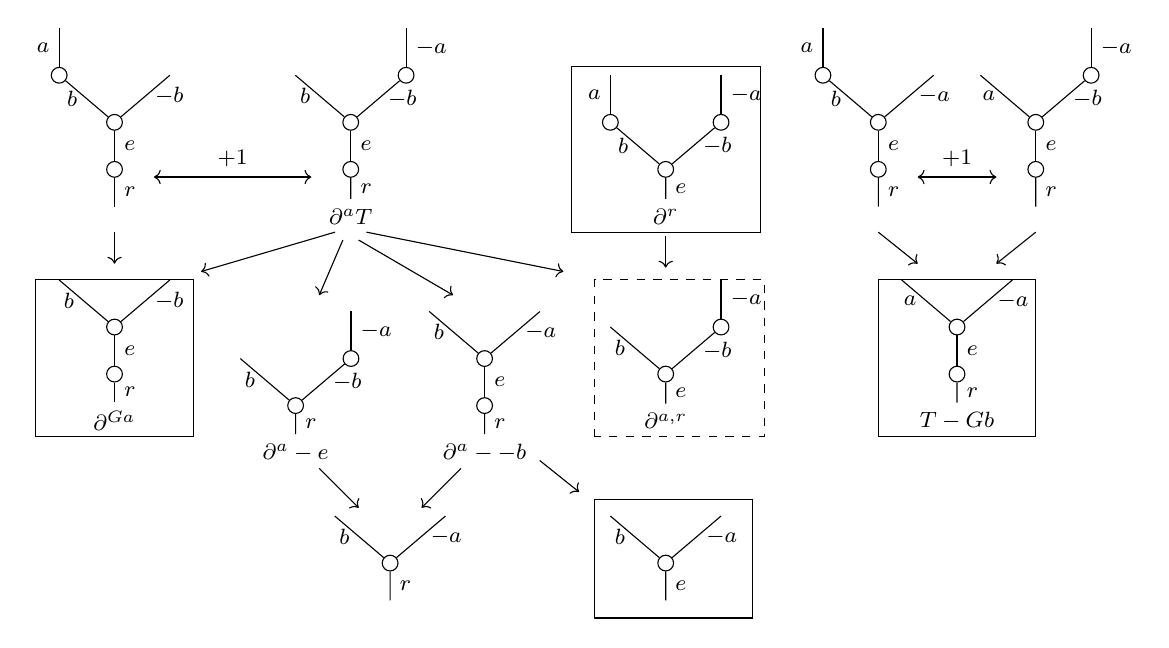
\begin{tikzpicture}[grow= up, level distance = 1.7em, every node/.style = {font=\footnotesize}]
                  \tikzstyle{level 2}=[sibling distance=4em]
                  \tikzstyle{level 3}=[sibling distance=4em]
                  \node (Paa) {}
                  child{node [dummy] {}
                    child{node [dummy] {}
                      child{
                        edge from parent node [right] {$-b$}
                      }
                      child{node [dummy] {}
                        child{edge from parent node [left] {$a$}}
                        edge from parent node [left] {$b$}
                      }
                      edge from parent node [right] {$e$}
                    }
                    edge from parent node [right] {$r$}
                  };
                  \node (Pa) at (3,0) {$\partial^{a} T$}
                  child{node [dummy] {}
                    child{node [dummy] {}
                      child{node [dummy] {}
                        child{edge from parent node [right] {$-a$}}
                        edge from parent node [right] {$-b$}
                      }
                      child{
                        edge from parent node [left] {$b$}
                      }
                      edge from parent node [right] {$e$}
                    }
                    edge from parent node [right] {$r$}
                  };
                  \node (Pr) at (7,0){$\partial^r$}
                  child{node [dummy] {}
                    child{node [dummy] {}
                      child{edge from parent node [right] {$-a$}}
                      edge from parent node [right] {$-b$}
                    }
                    child{node [dummy] {}
                      child{edge from parent node [left] {$a$}}
                      edge from parent node [left] {$b$}
                    }
                    edge from parent node [right] {$e$}
                  };
                  \draw
                  (Pr)++(-1.2,-.2) rectangle ++(2.4,2.1);
                  \node (Tb) at (9.7,0){}
                  child{node [dummy] {}
                    child{node [dummy] {}
                      child{edge from parent node [right] {$-a$}}
                      child{node [dummy] {}
                        child{edge from parent node [left] {$a$}}
                        edge from parent node [left] {$b$}
                      }
                      edge from parent node [right] {$e$}
                    }
                    edge from parent node [right] {$r$}
                  };
                  \node (Tbb) at (11.7,0) {}
                  child{node [dummy] {}
                    child{node [dummy] {}
                      child{node [dummy] {}
                        child{edge from parent node [right] {$-a$}}
                        edge from parent node [right] {$-b$}
                      }
                      child{
                        edge from parent node [left] {$a$}
                      }
                      edge from parent node [right] {$e$}
                    }
                    edge from parent node [right] {$r$}
                  };
                  %%%%%%% --------- NEXT ROW -----------------------------
                  \node (PGa) at (0,-2.6) {$\partial^{G a}$}
                  child{node [dummy] {}
                    child{node [dummy] {}
                      child{
                        edge from parent node [right] {$-b$}
                      }
                      child{
                        edge from parent node [left] {$b$}
                      }
                      edge from parent node [right] {$e$}
                    }
                    edge from parent node [right] {$r$}
                  };
                  \draw
                  (PGa)++(-1,-.2) rectangle ++(2,2);
                  %
                  \node (TGb) at (10.7,-2.6) {$T - G b$}
                  child{node [dummy] {}
                    child{node [dummy] {}
                      child{
                        edge from parent node [right] {$-a$}
                      }
                      child{
                        edge from parent node [left] {$a$}
                      }
                      edge from parent node [right] {$e$}
                    }
                    edge from parent node [right] {$r$}
                  };
                  \draw
                  (TGb)++(-1,-.2) rectangle ++(2, 2);
                  % -------- other orbital face of \partial{a}
                  \node (Par) at (7,-2.6) {$\partial^{a,r}$}
                  child{node [dummy] {}
                    child{node [dummy] {}
                      child{edge from parent node [right] {$-a$}}
                      edge from parent node [right] {$-b$}
                    }
                    child{edge from parent node [left] {$b$}}
                    edge from parent node [right] {$e$}
                  };
                  \draw[dashed]
                  (Par)++(-.9,-.2) rectangle ++(2.15,2);
                  % ---------- other faces of \partial{a}
                  \node (Pae) at (2.3, -3) {$\partial^{a}-e$}
                  child{node [dummy] {}
                    child{node [dummy] {}
                      child{edge from parent node [right] {$-a$}}
                      edge from parent node [right] {$-b$}
                    }
                    child{edge from parent node [left] {$b$}
                    }
                    edge from parent node [right] {$r$}
                  };
                  \node (Pabb) at (4.7,-3) {$\partial^{a}-\set{-b}$}
                  child{node [dummy] {}
                    child{node [dummy] {}
                      child{edge from parent node [right] {$-a$}}
                      child{edge from parent node [left] {$b$}}
                      edge from parent node [right] {$e$}
                    }
                    edge from parent node [right] {$r$}
                  };
                  %%%% -------------------- next row --------------------
                  \node at (3.5, -5) {}
                  child{node [dummy] {}
                    child{edge from parent node [right] {$-a$}}
                    child{edge from parent node [left] {$b$}}
                    edge from parent node [right] {$r$}
                  };
                  \node (Parb) at (7,-5) {}
                  child{node [dummy] {}
                    child{edge from parent node [right] {$-a$}}
                    child{edge from parent node [left] {$b$}}
                    edge from parent node [right] {$e$}
                  };
                  \draw
                  (Parb)++(-.9,-.1) rectangle ++(2,1.5);
                  %%%% -------------------- edges ----------
                  % ---------- conjugates ----------
                  \draw[<->]
                  (Pa)++(-.5,.5) -- (.5,.5) node [midway,above] {$+1$};
                  \draw[<->]
                  (Tbb)++(-.5,.5) -- ++(-1,0) node [midway,above] {$+1$};
                  % faces
                  \draw[->]
                  (Paa)++(0,-.2) -- ++(0,-.4);
                  \draw[->]
                  (Pr)++(0,-.25) -- ++(0,-.4);
                  \draw[->]
                  (Tb)++(0,-.2) -- ++(.5,-.4);
                  \draw[->]
                  (Tbb)++(0,-.2) -- ++(-.5,-.4);
                  % ---------- faces of Pa
                  \draw[->]
                  (Pa)++(-.2,-.2) -- (1.1,-.7);
                  \draw[->]
                  (Pa)++(-.1,-.3) -- (2.6,-1);
                  \draw[->]
                  (Pa)++(.1,-.3) -- (4.3,-1);
                  \draw[->]
                  (Pa)++(.2,-.2) -- (5.7,-.7);
                  % ---------- faces of Pab
                  \draw[->]
                  (Pabb)++(-.3,-.2) -- ++(-.5,-.5);
                  \draw[->]
                  (Pabb)++(.7,-.1) -- ++(.5,-.4);
                  \draw[->]
                  (Pae)++(.3,-.2) -- ++(.5,-.5);
            \end{tikzpicture}
      \end{equation}
      
\end{document}



\begin{example}
      To set up an example comparing the orbital horns with regular inner horns, 
      let $G = C_4$ be the cyclic group with four elements, and consider the tree $T \in \Omega^G \subseteq \Omega_G$ below.
  \begin{equation}
        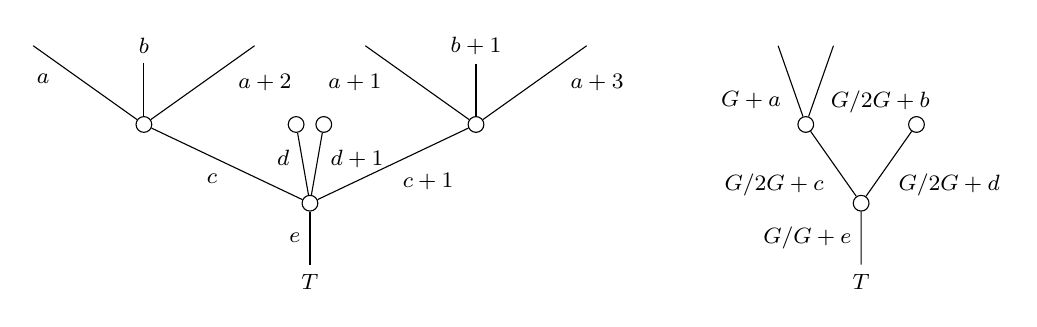
\begin{tikzpicture}[grow= up, auto, level distance = 1cm, every node/.style = {font=\footnotesize}]
              \tikzstyle{level 2}=[sibling distance=4em]
              \tikzstyle{level 3}=[sibling distance=4em]
              \node{$T$}
              child{node [dummy] {}%
                child{node [dummy] {}%
                  child{edge from parent node [swap,near end]{$a+3$}}
                  child{node {$b+1$}}
                  child{edge from parent node [near end] {$a+1$}}
                  edge from parent node [swap]{$c+1$}
                }
                child[sibling distance=1em]{node [dummy] {}
                  edge from parent node [swap,very near end]{$d+1$}
                }
                child[sibling distance=1em]{node [dummy] {}
                  edge from parent node [very near end]{$d$}
                }
                child{node [dummy] {}%
                  child{edge from parent node [swap, near end]{$a+2$}}
                  child{node {$b$}}
                  child{edge from parent node [near end] {$a$}}
                  edge from parent node {$c$}
                }
                edge from parent node {$e$}
              };
              \tikzstyle{level 3}=[sibling distance=2em]
              \node at (7,0){$T$}
              child{node [dummy] {}%
                child{node [dummy] {}
                  edge from parent node [swap]{$G/2G+d$}
                }
                child{node [dummy] {}%
                  child{edge from parent node [swap]{$G/2G + b$}}
                  child{edge from parent node {$G + a$}}
                  edge from parent node {$G/2G+c$}
                }
                edge from parent node {$G/G+e$}
              };
        \end{tikzpicture}
  \end{equation}
  The following are all proper faces of $T$ which are \textit{not} in the inner horn $\Lambda^{G e}[T]$:
  \begin{equation}
        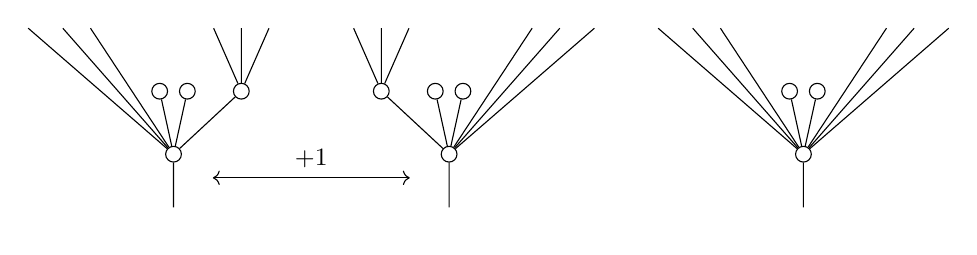
\begin{tikzpicture}
              [grow=up, level distance = .8cm, every node/.style={font=\small}]
              \tikzstyle{level 2}=[sibling distance=1.5em]
              \tikzstyle{level 3}=[sibling distance=1em]
              % -------------- PROPER FACES MISSING FROM \Lambda^{G e}[T] -----------------------------
              \node (Te) at (1,3) {}
              child{node [dummy] {}
                child[sibling distance=.7em]{node [dummy] {}
                  child{}
                  child{}
                  child{}
                }
                child[sibling distance=1em]{edge from parent [draw = none]}
                child[sibling distance=1em]{edge from parent [draw = none]}
                child[sibling distance=1em]{node [dummy] {}}
                child[sibling distance=1em]{node [dummy] {}}
                child[sibling distance=2em,level distance = 1.6cm]{}
                child[sibling distance=1.6em,level distance = 1.6cm]{}
                child[sibling distance=1.5em,level distance = 1.6cm]{}
              };
              \node (Tge) at (4.5,3) {}
              child{node [dummy] {}
                child[level distance = 1.6cm]{}
                child[sibling distance = 1.6em,level distance = 1.6cm]{}
                child[sibling distance = 2em, level distance = 1.6cm]{}
                child[sibling distance = 1em]{node [dummy] {}}
                child[sibling distance = 1em]{node [dummy] {}}
                child[sibling distance=1em]{edge from parent [draw = none]}
                child[sibling distance=1em]{edge from parent [draw = none]}
                child[sibling distance=.7em]{node [dummy] {}
                  child{}
                  child{}
                  child{}
                }
              };
              \draw[<->]
              (Te)+(.5,.5) -- +(3,.5) node [midway, above] {$+1$};
              \node (TGe) at (9,3) {}
              child{node [dummy] {}
                child[level distance = 1.6cm]{}
                child[sibling distance=1.6em,level distance = 1.6cm]{}
                child[sibling distance=2em,level distance = 1.6cm]{}
                child[sibling distance=1em]{node [dummy] {}}
                child[sibling distance=1em]{node [dummy] {}}
                child[sibling distance=2em,level distance = 1.6cm]{}
                child[sibling distance=1.6em,level distance = 1.6cm]{}
                child[sibling distance=1.5em,level distance = 1.6cm]{}
              };
        \end{tikzpicture}
  \end{equation}
  where the tree on the right is a face of both trees in the orbit on the left.
  Similarly, the maximal elements of $\Lambda^{G e}[T]$ are displayed in the top row below,
  while the second row displays the maximal elements of $\Lambda^{G e}_o[T]$;
  we observe that, in this particular case (where each orbit of vertices has at most two elements),
  these are all maximal subfaces of elements in the top row.
  For clarity, we have drawn using dashed lines the inner edges collapsed involving stumps.
    \begin{equation}
        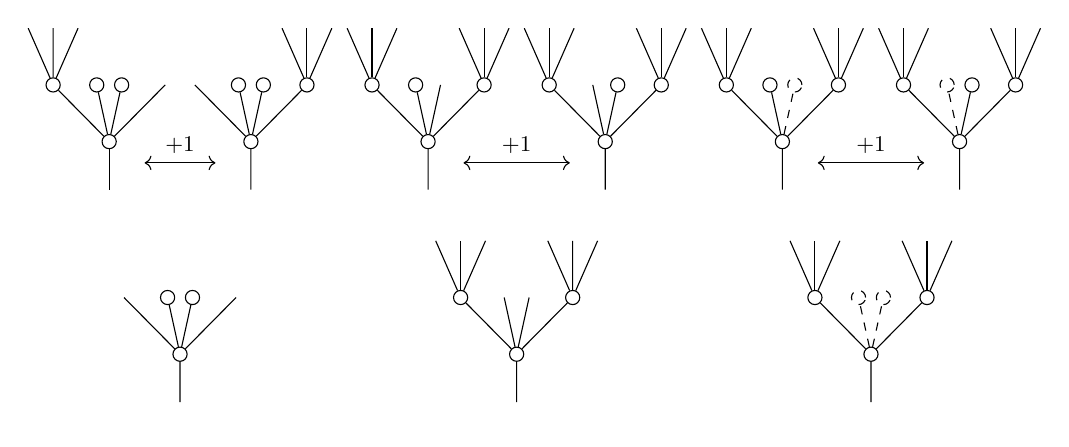
\begin{tikzpicture}
              [grow=up, level distance = .8cm, every node/.style={font=\small, transform shape},
              scale=0.9
              ]
              \tikzstyle{level 2}=[sibling distance=1.5em]
              \tikzstyle{level 3}=[sibling distance=1em]
              % -------------- MAXIMAL FACES OF \Lambda^{G e}[T] --------------------------------------
              \node (TC) {}
              child{node [dummy] {}
                child{}
                child[sibling distance=1em]{node [dummy] {}}
                child[sibling distance=1em]{node [dummy] {}}
                child{node [dummy] {}%
                  child{}
                  child{}
                  child{}
                }
              };
              \node (TgC) at (2,0) {}
              child{node [dummy] {}
                child{node [dummy] {}
                  child{}
                  child{}
                  child{}
                }
                child[sibling distance=1em]{node [dummy] {}}
                child[sibling distance=1em]{node [dummy] {}}
                child{}
              };
              \draw[<->]
              (TC)+(.5,.5) -- +(1.5,.5) node [midway, above] {$+1$};
              \node (TCd) at (4.5,0) {}
              child{node [dummy] {}
                child{node [dummy] {}
                  child{}
                  child{}
                  child{}
                }
                child[sibling distance=1em]{}
                child[sibling distance=1em]{node [dummy] {}}
                child{node [dummy] {}
                  child{}
                  child{}
                  child{}
                }
              };
              \node (TgCd) at (7,0) {}
              child{node [dummy] {}
                child{node [dummy] {}
                  child{}
                  child{}
                  child{}
                }
                child[sibling distance=1em]{node [dummy] {}}
                child[sibling distance=1em]{}
                child{node [dummy] {}
                  child{}
                  child{}
                  child{}
                }
              };
              \draw[<->]
              (TCd)+(.5,.5) -- +(2,.5) node [midway, above] {$+1$};
              \node (Td) at (9.5,0) {}
              child{node [dummy] {}
                child{node [dummy] {}
                  child{}
                  child{}
                  child{}
                }
                child[sibling distance=1em]{node [dummy, dashed] {}
                  edge from parent [dashed]
                }
                child[sibling distance=1em]{node [dummy] {}}
                child{node [dummy] {}
                  child{}
                  child{}
                  child{}
                }
              };
              \node (Tgd) at (12,0) {}
              child{node [dummy] {}
                child{node [dummy] {}
                  child{}
                  child{}
                  child{}
                }
                child[sibling distance=1em]{node [dummy] {}}
                child[sibling distance=1em]{node [dummy, dashed] {}
                  edge from parent [dashed]
                }
                child{node [dummy] {}
                  child{}
                  child{}
                  child{}
                }
              };
              \draw[<->]
              (Td)+(.5,.5) -- +(2,.5) node [midway, above] {$+1$};
              % --------- Maximal Faces in $\Lambda^{G e}_o[T]$ ---------------------------------------%%%%%
              \node (TGC) at (1, -3) {}
              child{node [dummy] {}
                child{}
                child[sibling distance=1em]{node [dummy] {}}
                child[sibling distance=1em]{node [dummy] {}}
                child{}
              };
              \node (TGCd) at (5.75,-3) {}
              child{node [dummy] {}
                child{node [dummy] {}
                  child{}
                  child{}
                  child{}
                }
                child[sibling distance=1em]{}
                child[sibling distance=1em]{}
                child{node [dummy] {}
                  child{}
                  child{}
                  child{}
                }
              };
              % \node (TB) at (7.5,-3) {}
              % child{node [dummy] {}
              %   child{}
              %   child{}
              %   child{}
              %   edge from parent node [left] {$e$}
              % };
              % \node (TgB) at (9,-3) {}
              % child{node [dummy] {}
              %   child{}
              %   child{}
              %   child{}
              %   edge from parent node [right] {$e+1$}
              % };
              % \draw[<->]
              % (TB)+(.3,.5) -- +(1.2,.5) node [midway,above] {$+1$};
              \node (TGd) at (10.75,-3) {}
              child{node [dummy] {}
                child{node [dummy] {}
                  child{}
                  child{}
                  child{}
                }
                child[sibling distance=1em]{node [dummy, dashed] {}
                  edge from parent [dashed]
                }
                child[sibling distance=1em]{node [dummy, dashed] {}
                  edge from parent [dashed]
                }
                child{node [dummy] {}
                  child{}
                  child{}
                  child{}
                }
              };
        \end{tikzpicture}
  \end{equation}
  However, these orbital faces are certainly \textit{not} the only subfaces of the top row above.
  In particular, the following is a minimal face in $\Lambda^{G e}[T]$ not in the orbital horn $\Lambda^{G e}_o[T]$.
  \begin{equation}
        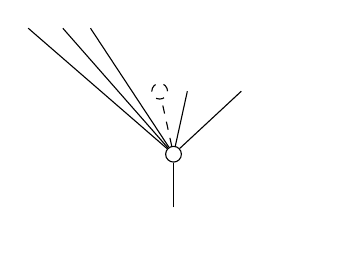
\begin{tikzpicture}
              [grow=up, level distance=.8cm, every node/.style={font=\small}]
              \tikzstyle{level 2}=[sibling distance=2em]
              \tikzstyle{level 3}=[sibling distance=1em]
              \node{}
              child{node [dummy] {}
                child[sibling distance=.7em]{}
                child{edge from parent [draw = none]}
                child{edge from parent [draw = none]}
                child[sibling distance=1em]{}
                child[sibling distance=1em]{node [dummy, dashed] {}
                  edge from parent [dashed]
                }                
                child[sibling distance=2em,level distance = 1.6cm]{}
                child[sibling distance=1.6em,level distance = 1.6cm]{}
                child[sibling distance=1.5em,level distance = 1.6cm]{}
              };
        \end{tikzpicture}
  \end{equation}
  
        
  % \begin{equation}
  %       \begin{tikzpicture}
  %             [grow=up, level distance = .8cm, every node/.style={font=\small}]
  %             \tikzstyle{level 2}=[sibling distance=4em]
  %             \tikzstyle{level 3}=[sibling distance=2em]
  %             \node{}
  %             child{node [dummy] {}%
  %               child{node [dummy] {}%
  %                 child{edge from parent node [swap, right]{$b+1$}}
  %                 child{node [label={[label distance=-.2cm]90:$a+3$}]{}}
  %                 child{edge from parent node [left]{$a+1$}}
  %                 edge from parent node [auto, swap]{$c+1$}
  %               }
  %               child[sibling distance=1em]{edge from parent node [right,near end]{$d+1$}}
  %               child[sibling distance=1em]{edge from parent node [left, near end]{$d$}}
  %               child{node [dummy] {}%
  %                 child{edge from parent node [auto, swap]{$b$}}
  %                 child{node [label={[label distance=-.2cm]90:$a+2$}]{}}
  %                 child{edge from parent node [auto]{$a$}}
  %                 edge from parent node [auto]{$c$}
  %               }
  %               edge from parent node [right]{$e$}
  %             };
  %             \tikzstyle{level 2}=[sibling distance=2.5em]
  %             \node at (-5,-2){}
  %             child{node [dummy] {}%
  %               child[sibling distance=1.5em]{node [dummy] {}%
  %                 child{edge from parent node [auto, swap]{$b+1$}}
  %                 child{node [label={[label distance=-.2cm]90:$a+3$}]{}}
  %                 child{edge from parent node [left]{$a+1$}}
  %                 edge from parent node [auto, swap]{$c+1$}
  %               }
  %               child{edge from parent [draw=none]}
  %               child{edge from parent [draw=none]}
  %               child[sibling distance=1em]{edge from parent node [right,near end]{$d+1$}}
  %               child[sibling distance=1em]{edge from parent node [left,near end]{$d$}}
  %               child{edge from parent [draw=none]}
  %               child[level distance = 1.2cm]{edge from parent node [auto, swap]{$b$}}
  %               child[level distance = 1.2cm]{node [label={[label distance=-.2cm]90:$a+2$}]{}}
  %               child[level distance = 1.2cm]{edge from parent node [auto]{$a$}}
  %               edge from parent node [right]{$e$}
  %             };
  %             \node at (5,-2){}
  %             child{node [dummy] {}%
  %               child[level distance = 1.2cm]{edge from parent node [auto, swap]{$b+1$}}
  %               child[level distance = 1.2cm]{node [label={[label distance=-.2cm]90:$a+3$}]{}}
  %               child[level distance = 1.2cm]{edge from parent node [left, very near end]{$a+1$}}
  %               child{edge from parent [draw=none]}
  %               child{edge from parent [draw=none]}
  %               child[sibling distance=1em]{edge from parent node [right,near end]{$d+1$}}
  %               child[sibling distance=1em]{edge from parent node [left,near end]{$d$}}
  %               child{edge from parent [draw=none]}
  %               child[sibling distance=1.5em]{node [dummy] {}%
  %                 child{edge from parent node [auto, swap, near end]{$b$}}
  %                 child{node [label={[label distance=-.2cm]90:$a+2$}] {}}
  %                 child{edge from parent node [auto, near end]{$a$}}
  %                 edge from parent node [auto]{$c$}
  %               }
  %               edge from parent node [right]{$e$}
  %             };
  %             \tikzstyle{level 2}=[sibling distance=1.5em]
  %             \node at (0,-4){}
  %             child{node [dummy] {}%
  %               child[level distance = 1cm]{edge from parent node [auto, swap, near end]{$b+1$}}
  %               child[level distance = 1cm]{node [label={[label distance=-.2cm]90:$a+3$}]{}}
  %               child[level distance = 1cm]{edge from parent node [auto, very near end]{$a+1$}}
  %               child{edge from parent [draw=none]}
  %               child{edge from parent [draw=none]}
  %               child[sibling distance=1em]{edge from parent node [near end,right]{$d+1$}}
  %               child[sibling distance=1em]{edge from parent node [near end, left]{$d$}}
  %               child{edge from parent [draw=none]}
  %               child{edge from parent [draw=none]}
  %               child[level distance = 1cm]{edge from parent node [auto, swap, near end]{$b$}}
  %               child[level distance = 1cm]{node [label={[label distance=-.2cm]90:$a+2$}]{}}
  %               child[level distance = 1cm]{edge from parent node [auto, near end]{$a$}}
  %               edge from parent node [right]{$e$}
  %             };
  %       \end{tikzpicture}
  % \end{equation}
\end{example}

\end{document}
